
\documentclass[10pt,a4paper]{article}
\usepackage[T1]{fontenc}
\usepackage[utf8]{inputenc}
\usepackage{lmodern}
\usepackage[margin=17mm]{geometry}
\usepackage{amsmath,amssymb}
\usepackage{graphicx}
\usepackage{longtable,booktabs,array,calc}
\usepackage{etoolbox}
\usepackage{upquote}
\usepackage{xcolor}
\usepackage{xurl}
\usepackage[unicode,hidelinks]{hyperref}
\setcounter{secnumdepth}{-\maxdimen}
\setlength{\parindent}{0pt}
\setlength{\parskip}{5pt}
\setlength{\emergencystretch}{3em}
\providecommand{\tightlist}{\setlength{\itemsep}{0pt}\setlength{\parskip}{0pt}}
\AtBeginEnvironment{longtable}{\footnotesize\setlength{\tabcolsep}{4pt}\renewcommand{\arraystretch}{1.18}}
\newcommand{\missingmarketimage}{%
\begin{center}\fbox{\parbox{0.90\linewidth}{\centering
U.S. Robotaxi Markets by Company\\[6pt]
\texttt{images/robotaxi\_market.png}\\[4pt]
\small The image referenced in the source was not attached.
}}\end{center}}
\begin{document}
\hypertarget{u.s.-robotaxi-companies-and-operating-markets}{%
\section{U.S. Robotaxi Companies and Operating Markets}\label{u.s.-robotaxi-companies-and-operating-markets}}

\IfFileExists{images/robotaxi_market.png}{\begin{center}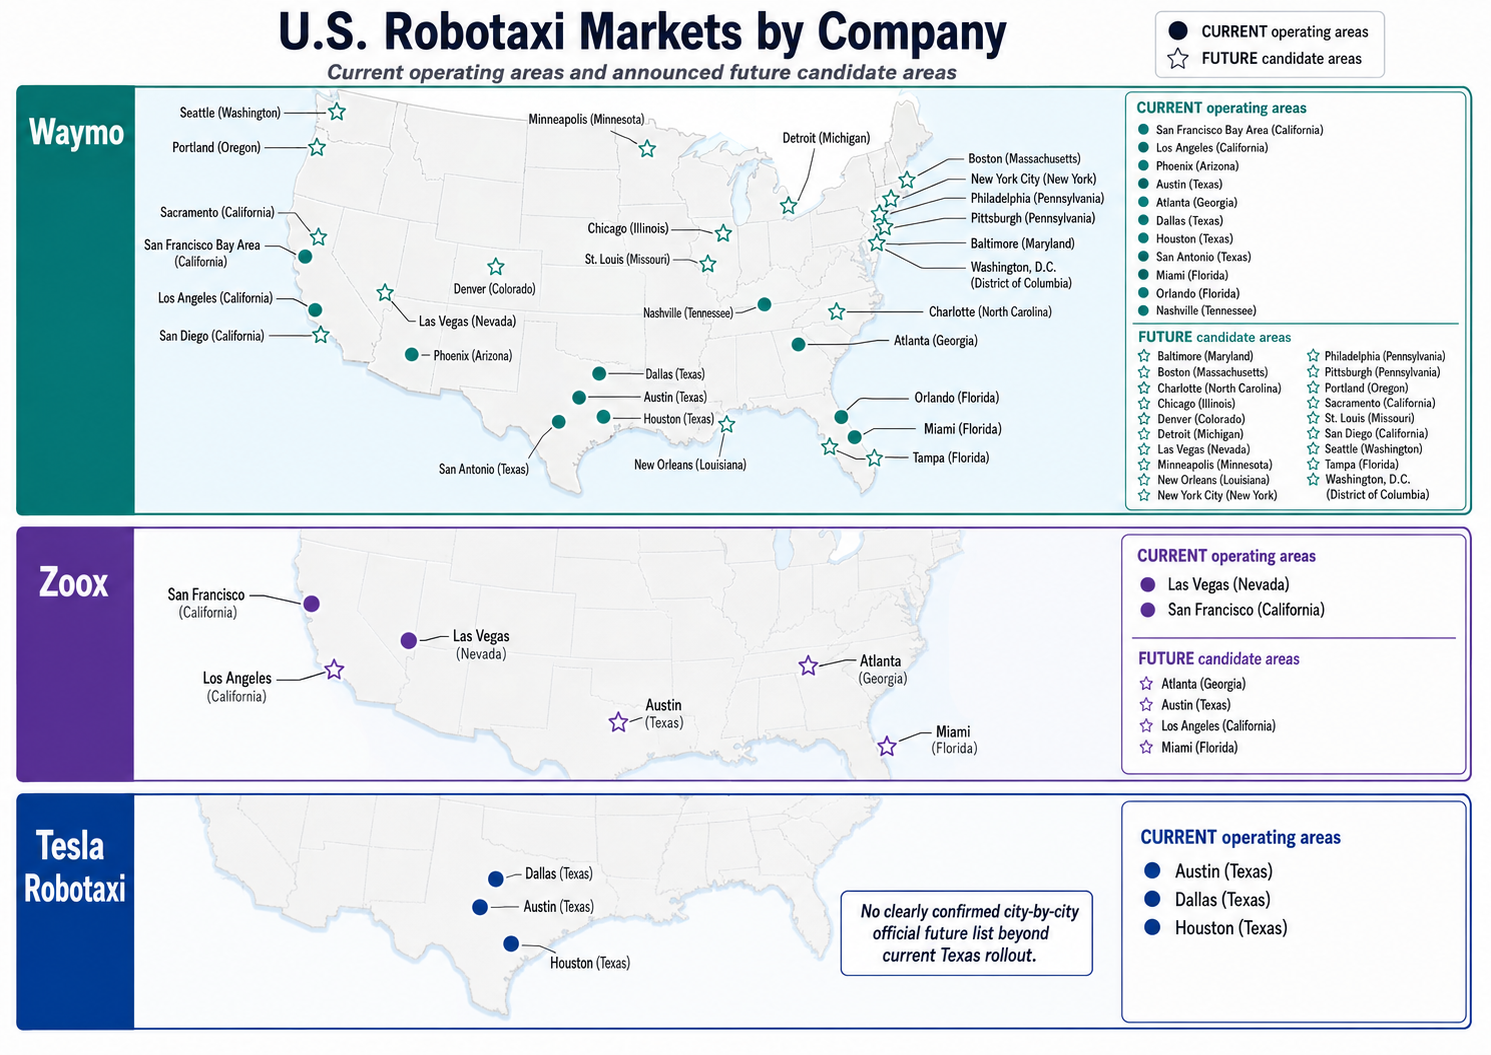
\includegraphics[width=0.95\linewidth]{images/robotaxi_market.png}\end{center}}{\missingmarketimage}

\hypertarget{waymo}{%
\subsection{1. Waymo}\label{waymo}}

\begin{itemize}
\item
  \textbf{Current operating areas:} Atlanta(Georgia), Austin(Texas), Dallas(Texas), Houston(Texas), Los Angeles(California), Miami(Florida), Nashville(Tennessee), Orlando(Florida), Phoenix(Arizona), San Antonio(Texas), San Francisco Bay Area(California)
\item
  \textbf{Future candidate operating areas:} Baltimore(Maryland), Boston(Massachusetts), Charlotte(North Carolina), Chicago(Illinois), Denver(Colorado), Detroit(Michigan), Las Vegas(Nevada), Minneapolis(Minnesota), New Orleans(Louisiana), New York City(New York), Philadelphia(Pennsylvania), Pittsburgh(Pennsylvania), Portland(Oregon), Sacramento(California), San Diego(California), Seattle(Washington), St.~Louis(Missouri), Tampa(Florida), Washington, D.C.(District of Columbia)
\item
  \textbf{Source:} \href{https://waymo.com/rides/}{Waymo --- Where Waymo Operates}
\end{itemize}

\begin{center}\rule{0.5\linewidth}{0.5pt}\end{center}

\hypertarget{zoox}{%
\subsection{2. Zoox}\label{zoox}}

\begin{itemize}
\item
  \textbf{Current operating areas:} Las Vegas(Nevada), San Francisco(California)
\item
  \textbf{Future candidate operating areas:} Atlanta(Georgia), Austin(Texas), Los Angeles(California), Miami(Florida)
\item
  \textbf{Source:} \href{https://zoox.com/where-to-ride}{Zoox --- Where to Ride}
\end{itemize}

\begin{quote}
\textbf{Note:} Zoox lists all six cities on its official ``Where to Ride'' page, but the service stages differ by city. Las Vegas and San Francisco are treated here as current public-rider markets, while Austin, Miami, Atlanta, and Los Angeles are classified as announced expansion or rollout markets.
\end{quote}

\begin{center}\rule{0.5\linewidth}{0.5pt}\end{center}

\hypertarget{tesla-robotaxi}{%
\subsection{3. Tesla Robotaxi}\label{tesla-robotaxi}}

\begin{itemize}
\item
  \textbf{Current operating areas:} Austin(Texas), Dallas(Texas), Houston(Texas)
\item
  \textbf{Future candidate operating areas:} No additional U.S. cities have been confirmed in a sufficiently clear, city-by-city official list.
\item
  \textbf{Sources:}

  \begin{itemize}
  \tightlist
  \item
    \href{https://www.tesla.com/robotaxi}{Tesla --- Robotaxi}
  \item
    \href{https://www.reuters.com/business/autos-transportation/tesla-rolls-out-robotaxis-dallas-houston-2026-04-18/}{Reuters --- Tesla expands Robotaxi service to Dallas and Houston}
  \item
    \href{https://www.reuters.com/business/autos-transportation/tesla-rolls-out-unsupervised-robotaxis-austin-2026-06-03/}{Reuters --- Tesla rolls out unsupervised Robotaxis in the Austin Metro area}
  \end{itemize}
\end{itemize}

\begin{quote}
\textbf{Note:} Tesla has expressed a broad intention to expand Robotaxi service across additional U.S. markets, but unlike Waymo, it does not currently provide a reliable official ``Up Next'' city list. Therefore, unconfirmed cities are excluded.
\end{quote}

\end{document}
